\chapter{Railway Network}

\resp{Merlo Federico}

This task aim is to create a network of the European railways and stations, extrapolating data from the 2019 version of EuroGlobalMap, in order to study numerically its robustness under cascading failures.

\section{Extraction of Data}


First of all we need to extrapolate the data relative to all the railways and stations tracked in the EuroGlobalMap (EGM). This data are stored in two shapefiles, one for the stations, of geometry Point, and one for the railways, of geometry Line. The idea is to reshape this data in the more usable format of the CSV. To do that it has been developed a code in R that can be found in the GitHub \cite{mygithub}. 
The outputs of this code are two CSV files, one for the stations and one for the railways. The station file contains all endpoints of the partitions of the railways. Therefore, not all nodes are stations but all stations are nodes. The station file has headers 'nodeID, latitude, longitude, nodeLabel, country\_ISO3' that specify the node ID, chosen at random, its latitude and longitude and, only if the node is a station, its Label, which is its name in the original language found as NAMN1 attribute in EGM, and the ISO3 code of the country it belongs to. 
The railways file contains all the partitions of the railway coded with their endpoints, 'nodeID\_from, nodeID\_to'.









\section{Robustness Study}

Now that we posses the CSV files, we can easily create the network of all the railways in Europe or in a single country (from AL to IS), if the EGM provided it. Consequently, we can analyse its robustness against cascading failures, following the Motter-Lai overload model. A code, reachable at the GitHub \cite{mygithub}, has been developed to implement this model considering three possible cascade causes: a random failure, a degree based attack or a betweenness based attack. In this model we use the parameter $\alpha$ to define every node's threshold as $C_i = (1+\alpha)L_i$ with $L_i$ the node's initial betweenness centrality.

Due to the lack of resources, the study of the cascade caused by a random failure, which would require to run the simulation over many instances to have enough statistics, has been neglected here, although the functions to do it have been implemented nonetheless in the code.
Instead, the study of the degree and betweenness based attack have been implemented to the exemplary networks of the German and Danish railways.






\begin{figure}[h!t]
\centering

\subfigure[]{
    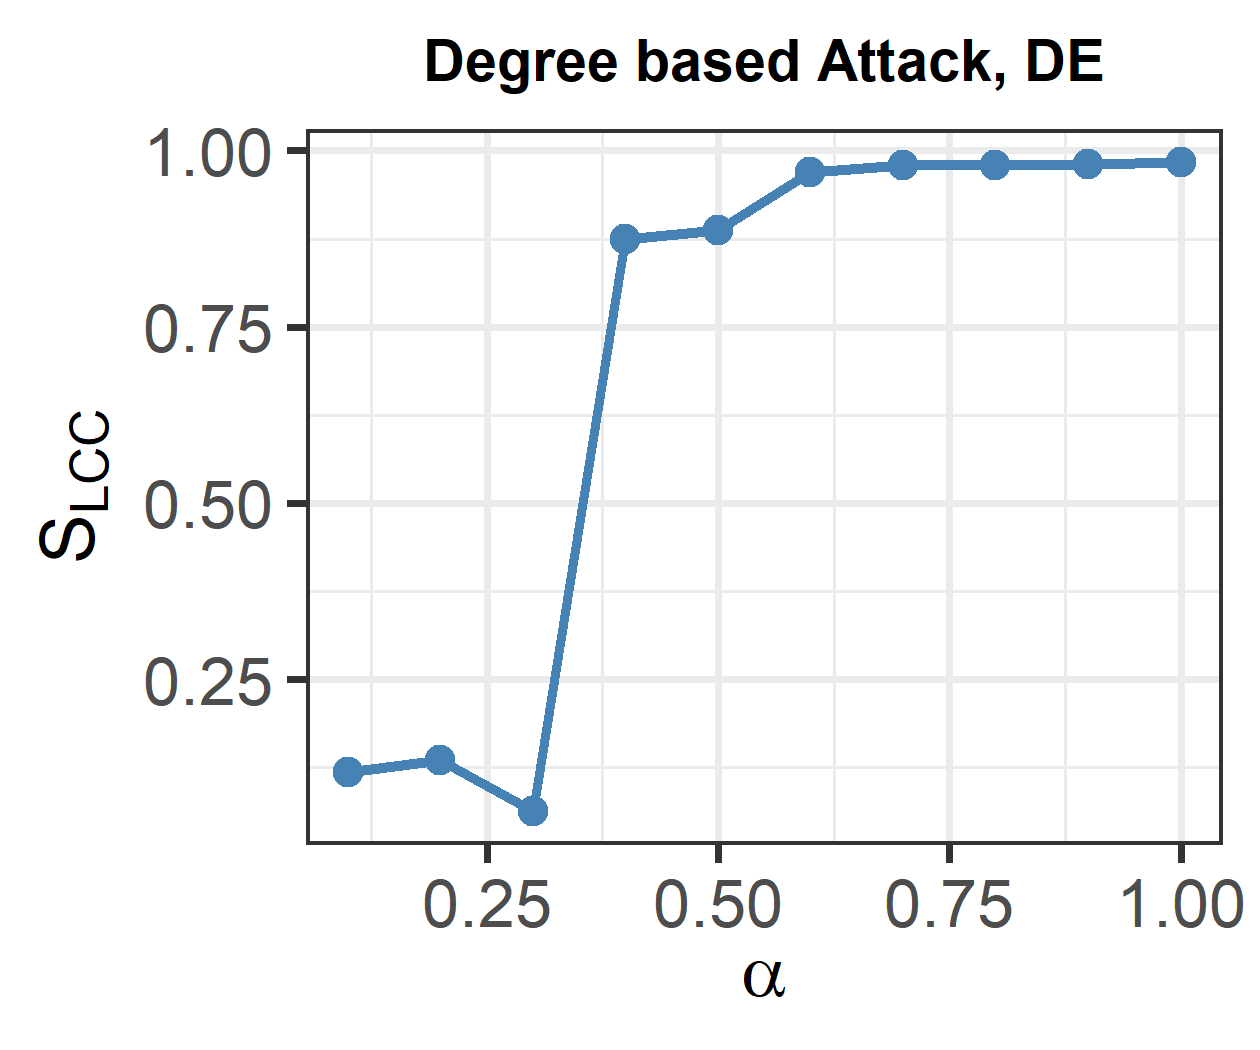
\includegraphics[width=0.47\textwidth]{images/DE_lcc_deg.png}
}
\subfigure[]{
    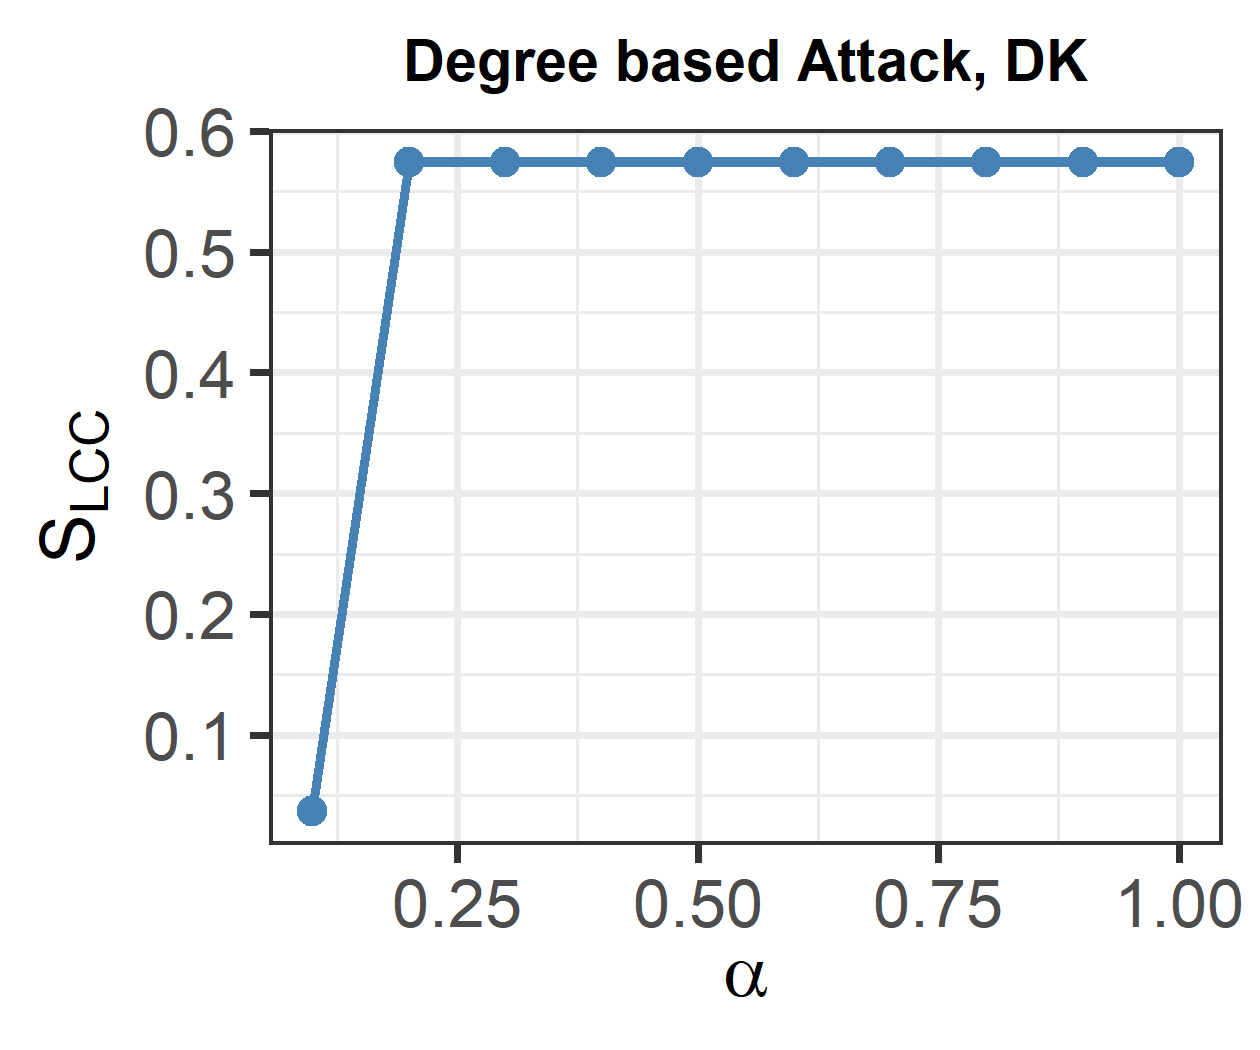
\includegraphics[width=0.47\textwidth]{images/DK_lcc_deg.png}
}

\caption{\textit{\small{Study of the size of the LCC for the German (a) and Danish (b) Railways Network over various $\alpha$ values, after degree based attack.}}}
\label{fig:deg}
\end{figure}





\begin{figure}[h!t]
\centering

\subfigure[]{
    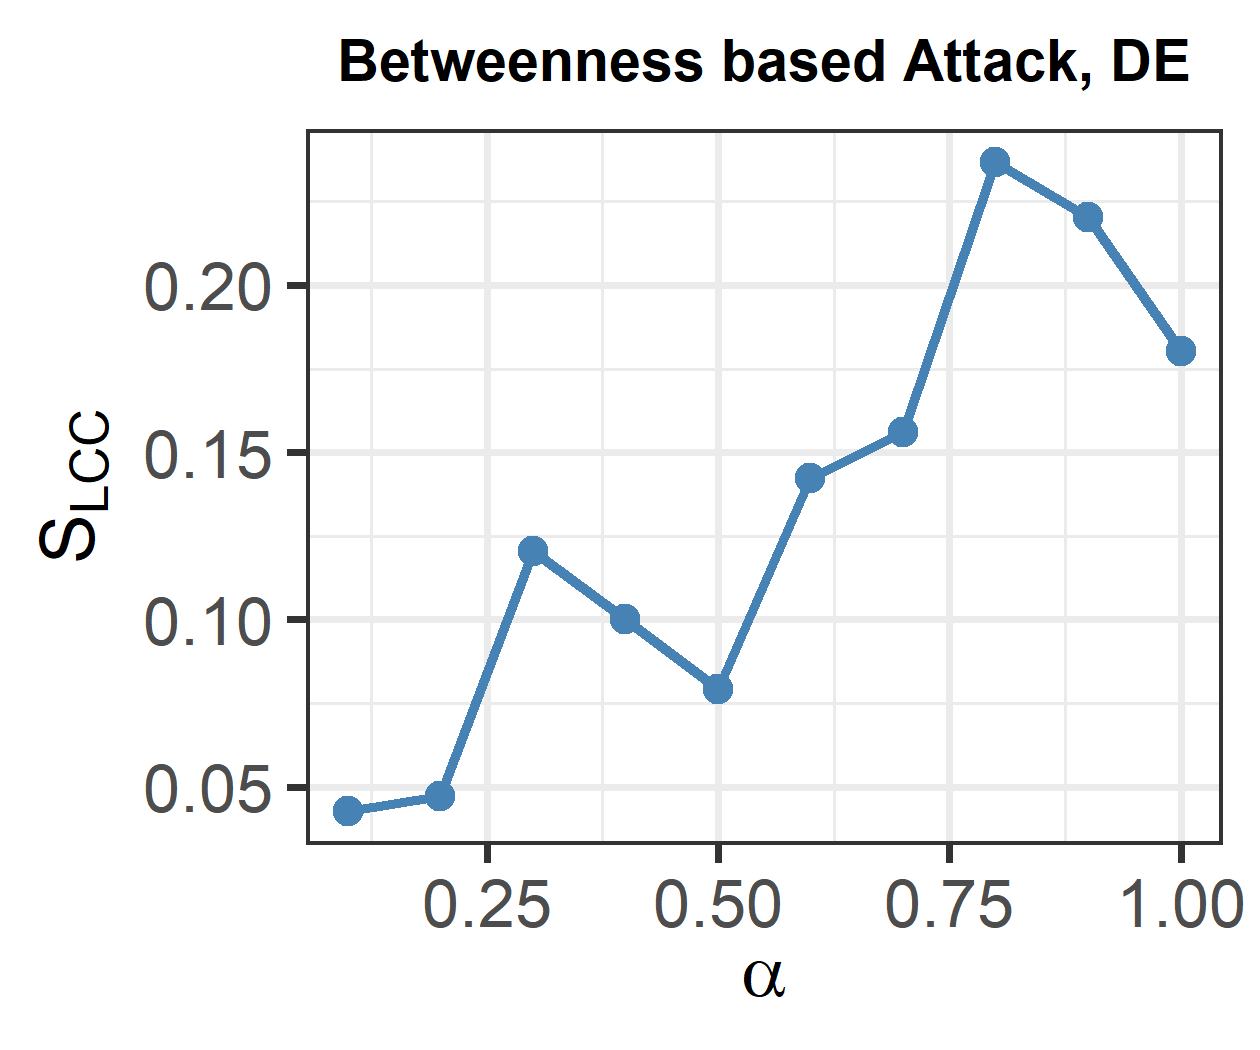
\includegraphics[width=0.47\textwidth]{images/DE_lcc_betw.png}
}
\subfigure[]{
    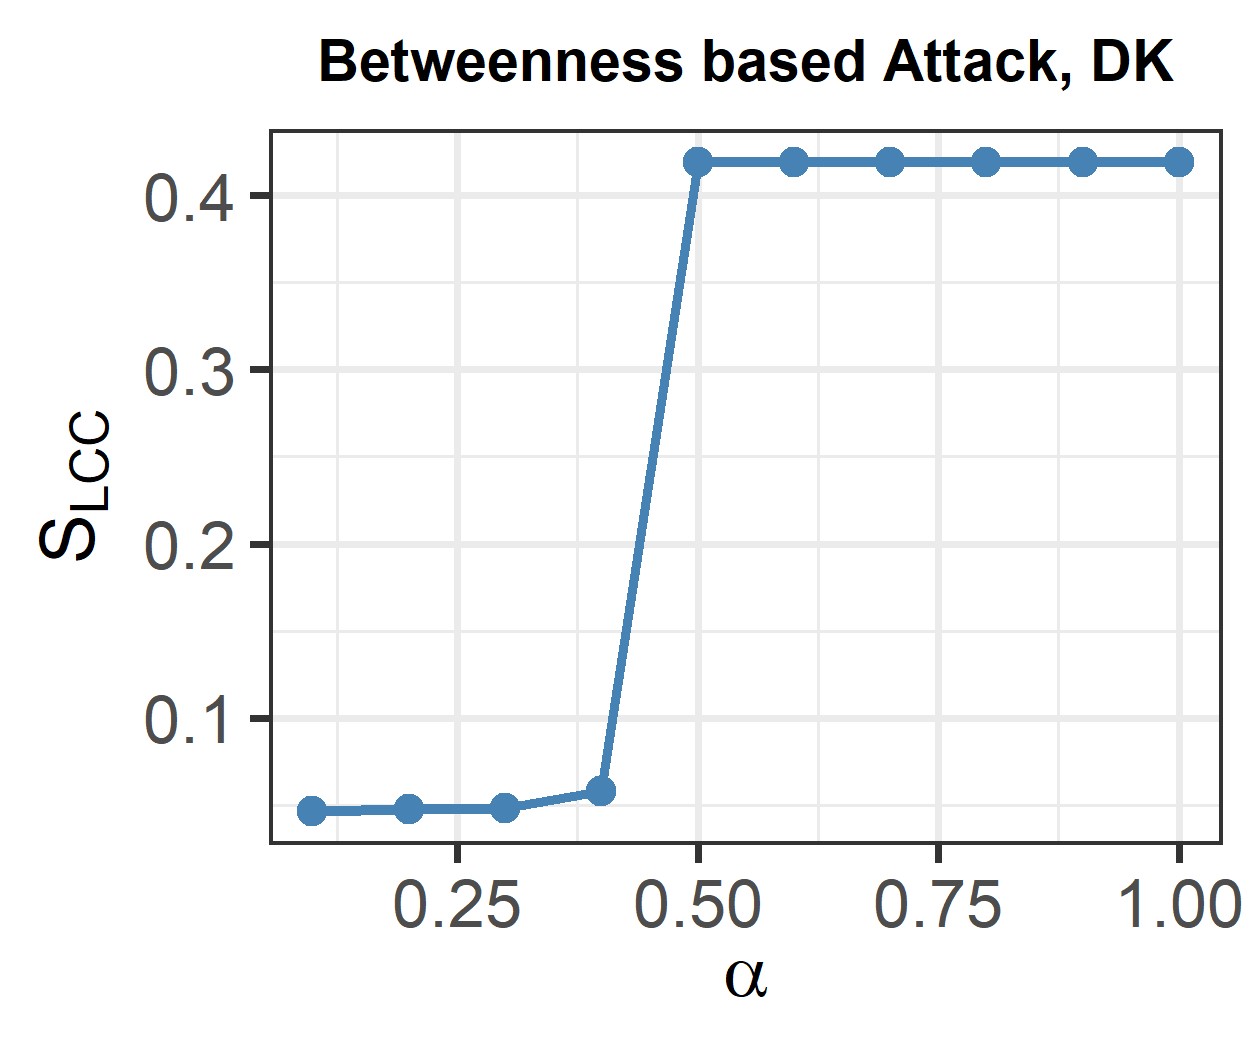
\includegraphics[width=0.47\textwidth]{images/DK_lcc_betw.png}
}

\caption{\textit{\small{Study of the size of the LCC for the  German (a) and Danish (b) Railways Network over various $\alpha$ values, after betweenness based attack.}}}
\label{fig:betw}
\end{figure}




The figure \ref{fig:deg} and \ref{fig:betw} show the variation of the size of the remaining Largest Connected Component for the two networks after a degree and a betweenness based attack, respectively. Notice that in this study we count as nodes also the simple endpoints of a railway's partitions, not only the Stations. This means that we study the failure of not only the stations but also of random points in the railways, like if, in a real world situation, a tree fell on the rails, for example. From this study we can see that attacking the highest degree node seems to affect more the small network of Denmark rather than the vast German one. Vice versa, attacking the node with highest betweenness damages more the German railway rather than the Danish one.
Also it is visible a non-monotonic behaviour of the size of the LCC, for increasing $\alpha$, in the German network. Having a slightly higher tolerance to overload sometimes seems to damage more the network. 


\newpage

\section{Appendix}


\begin{figure}[h!t]
\centering
    
    \subfigure{
    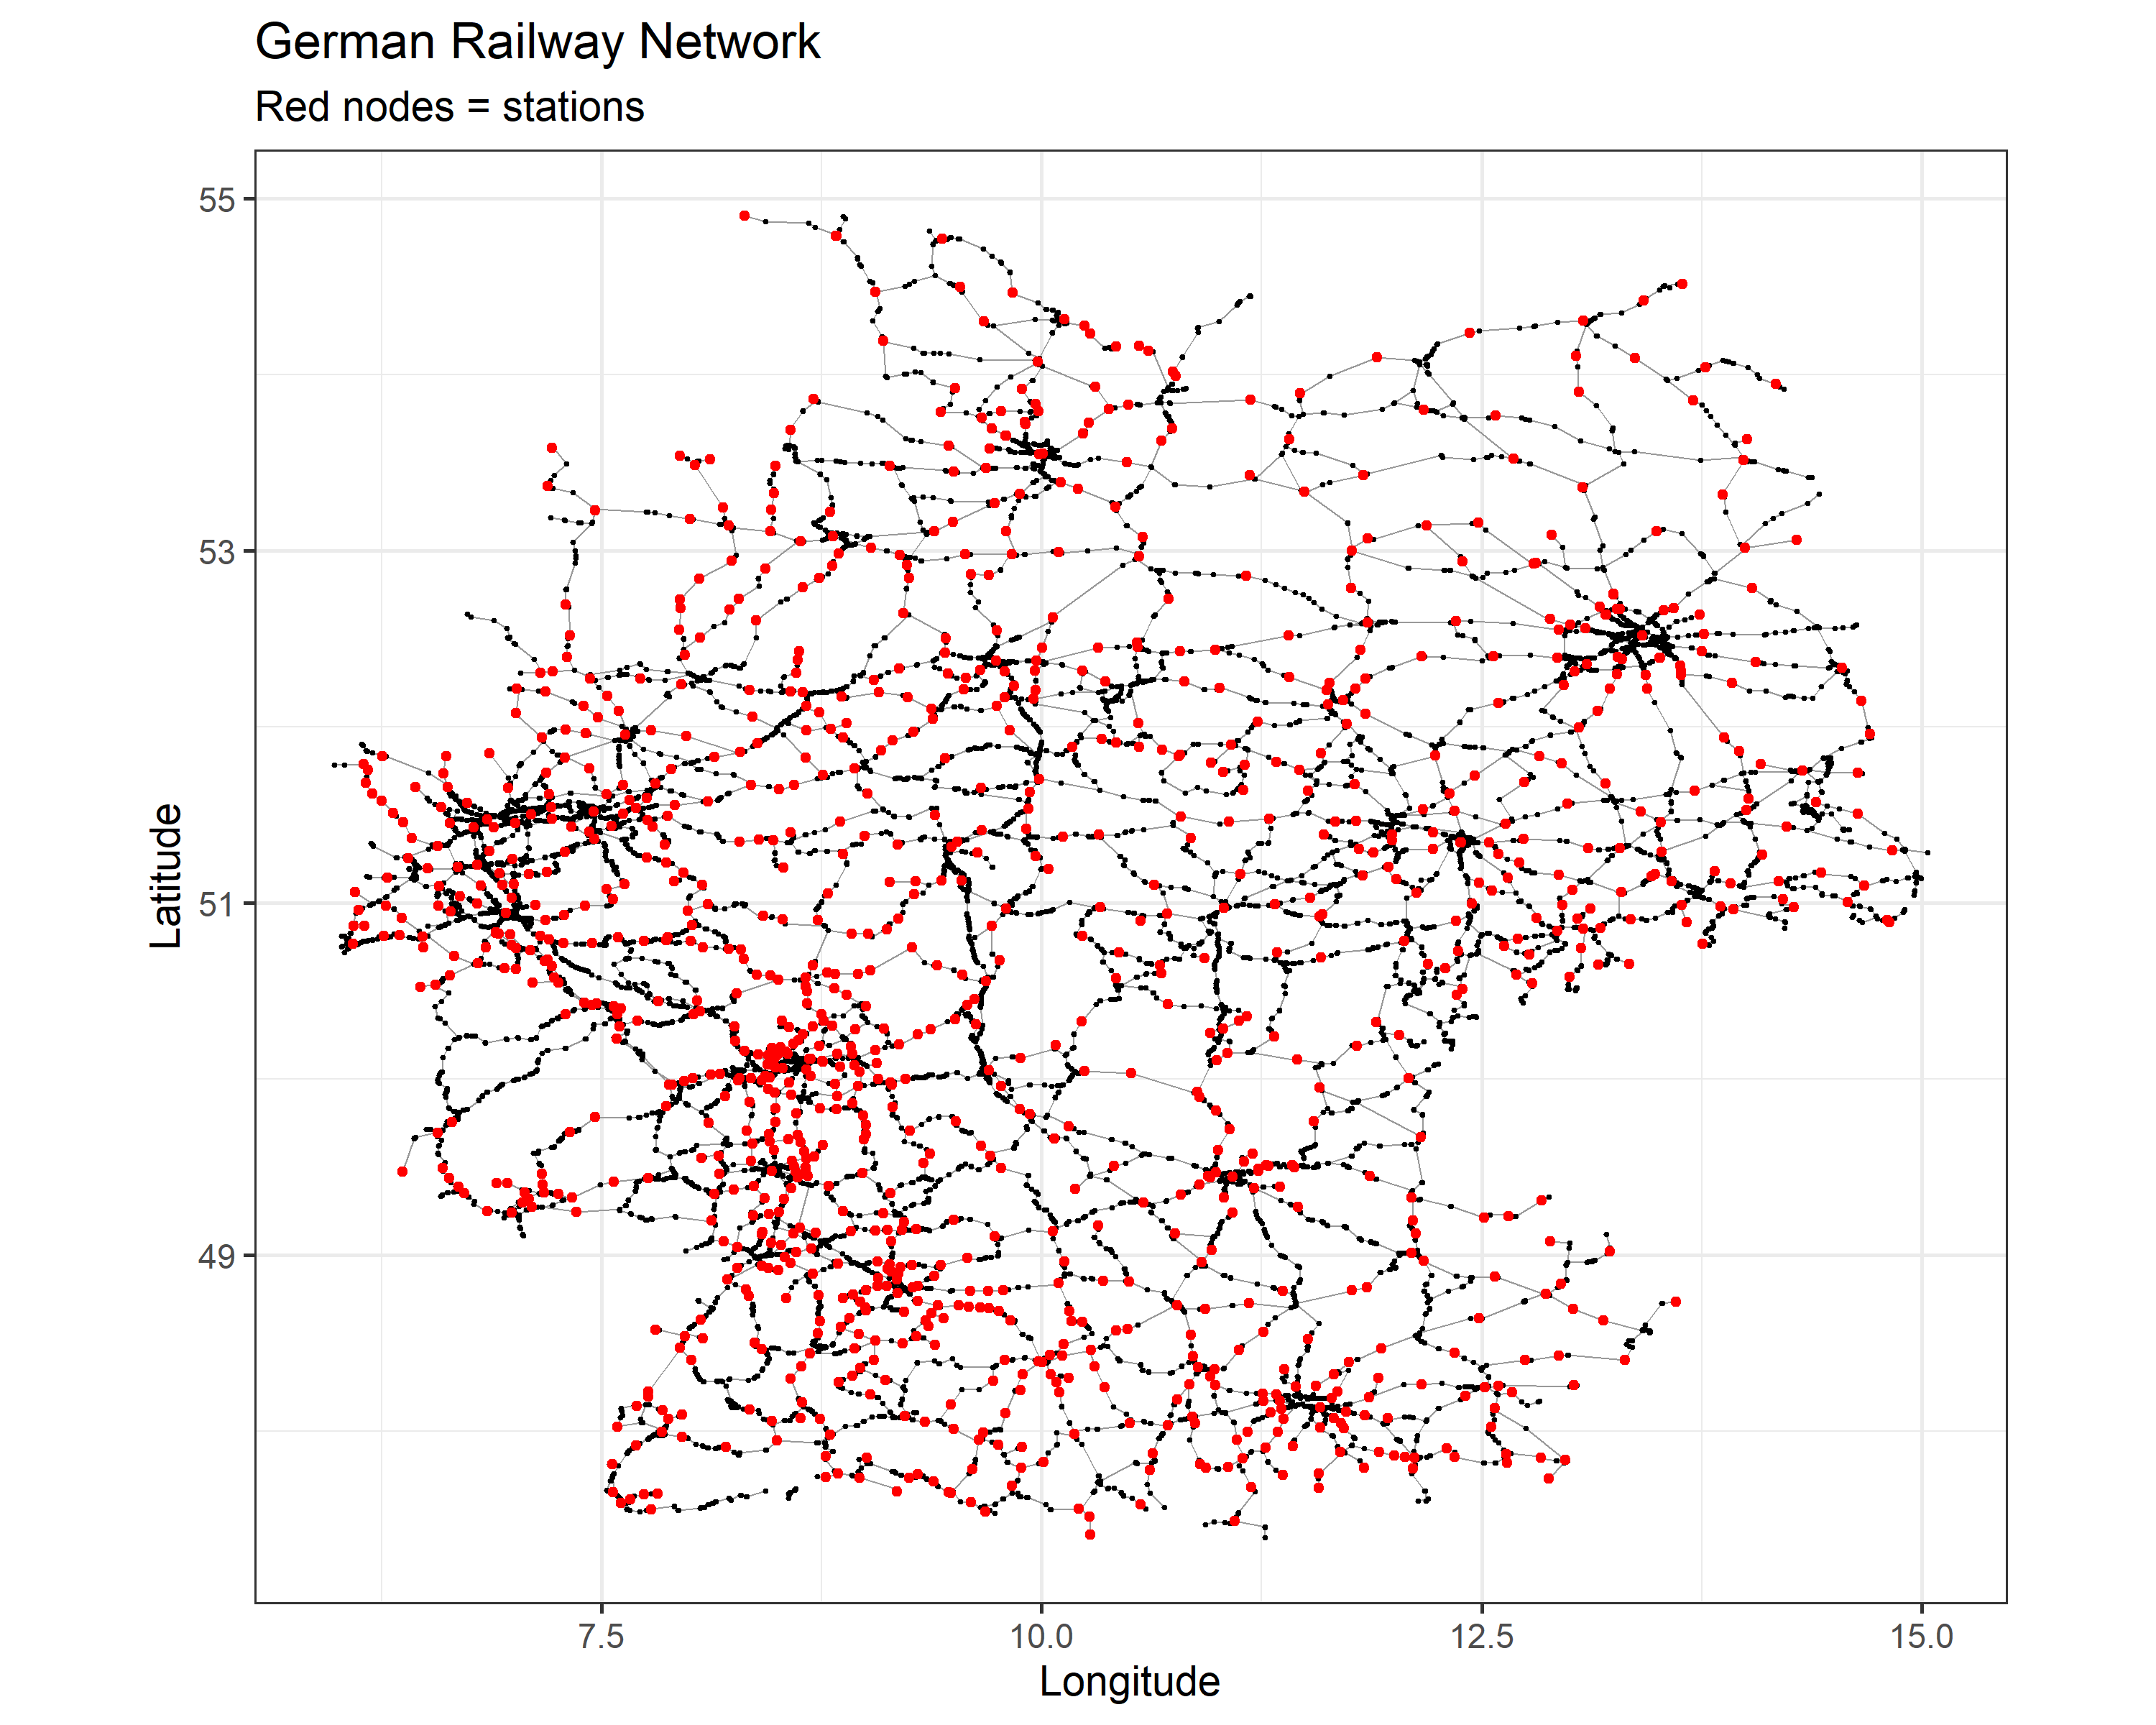
\includegraphics[width=1\textwidth]{images/railway_network_DE.png}
    }


    \caption{German Railways Network}
    \label{fig:de_net}
\end{figure}




\begin{figure}[h!t]
\centering

        \subfigure{
    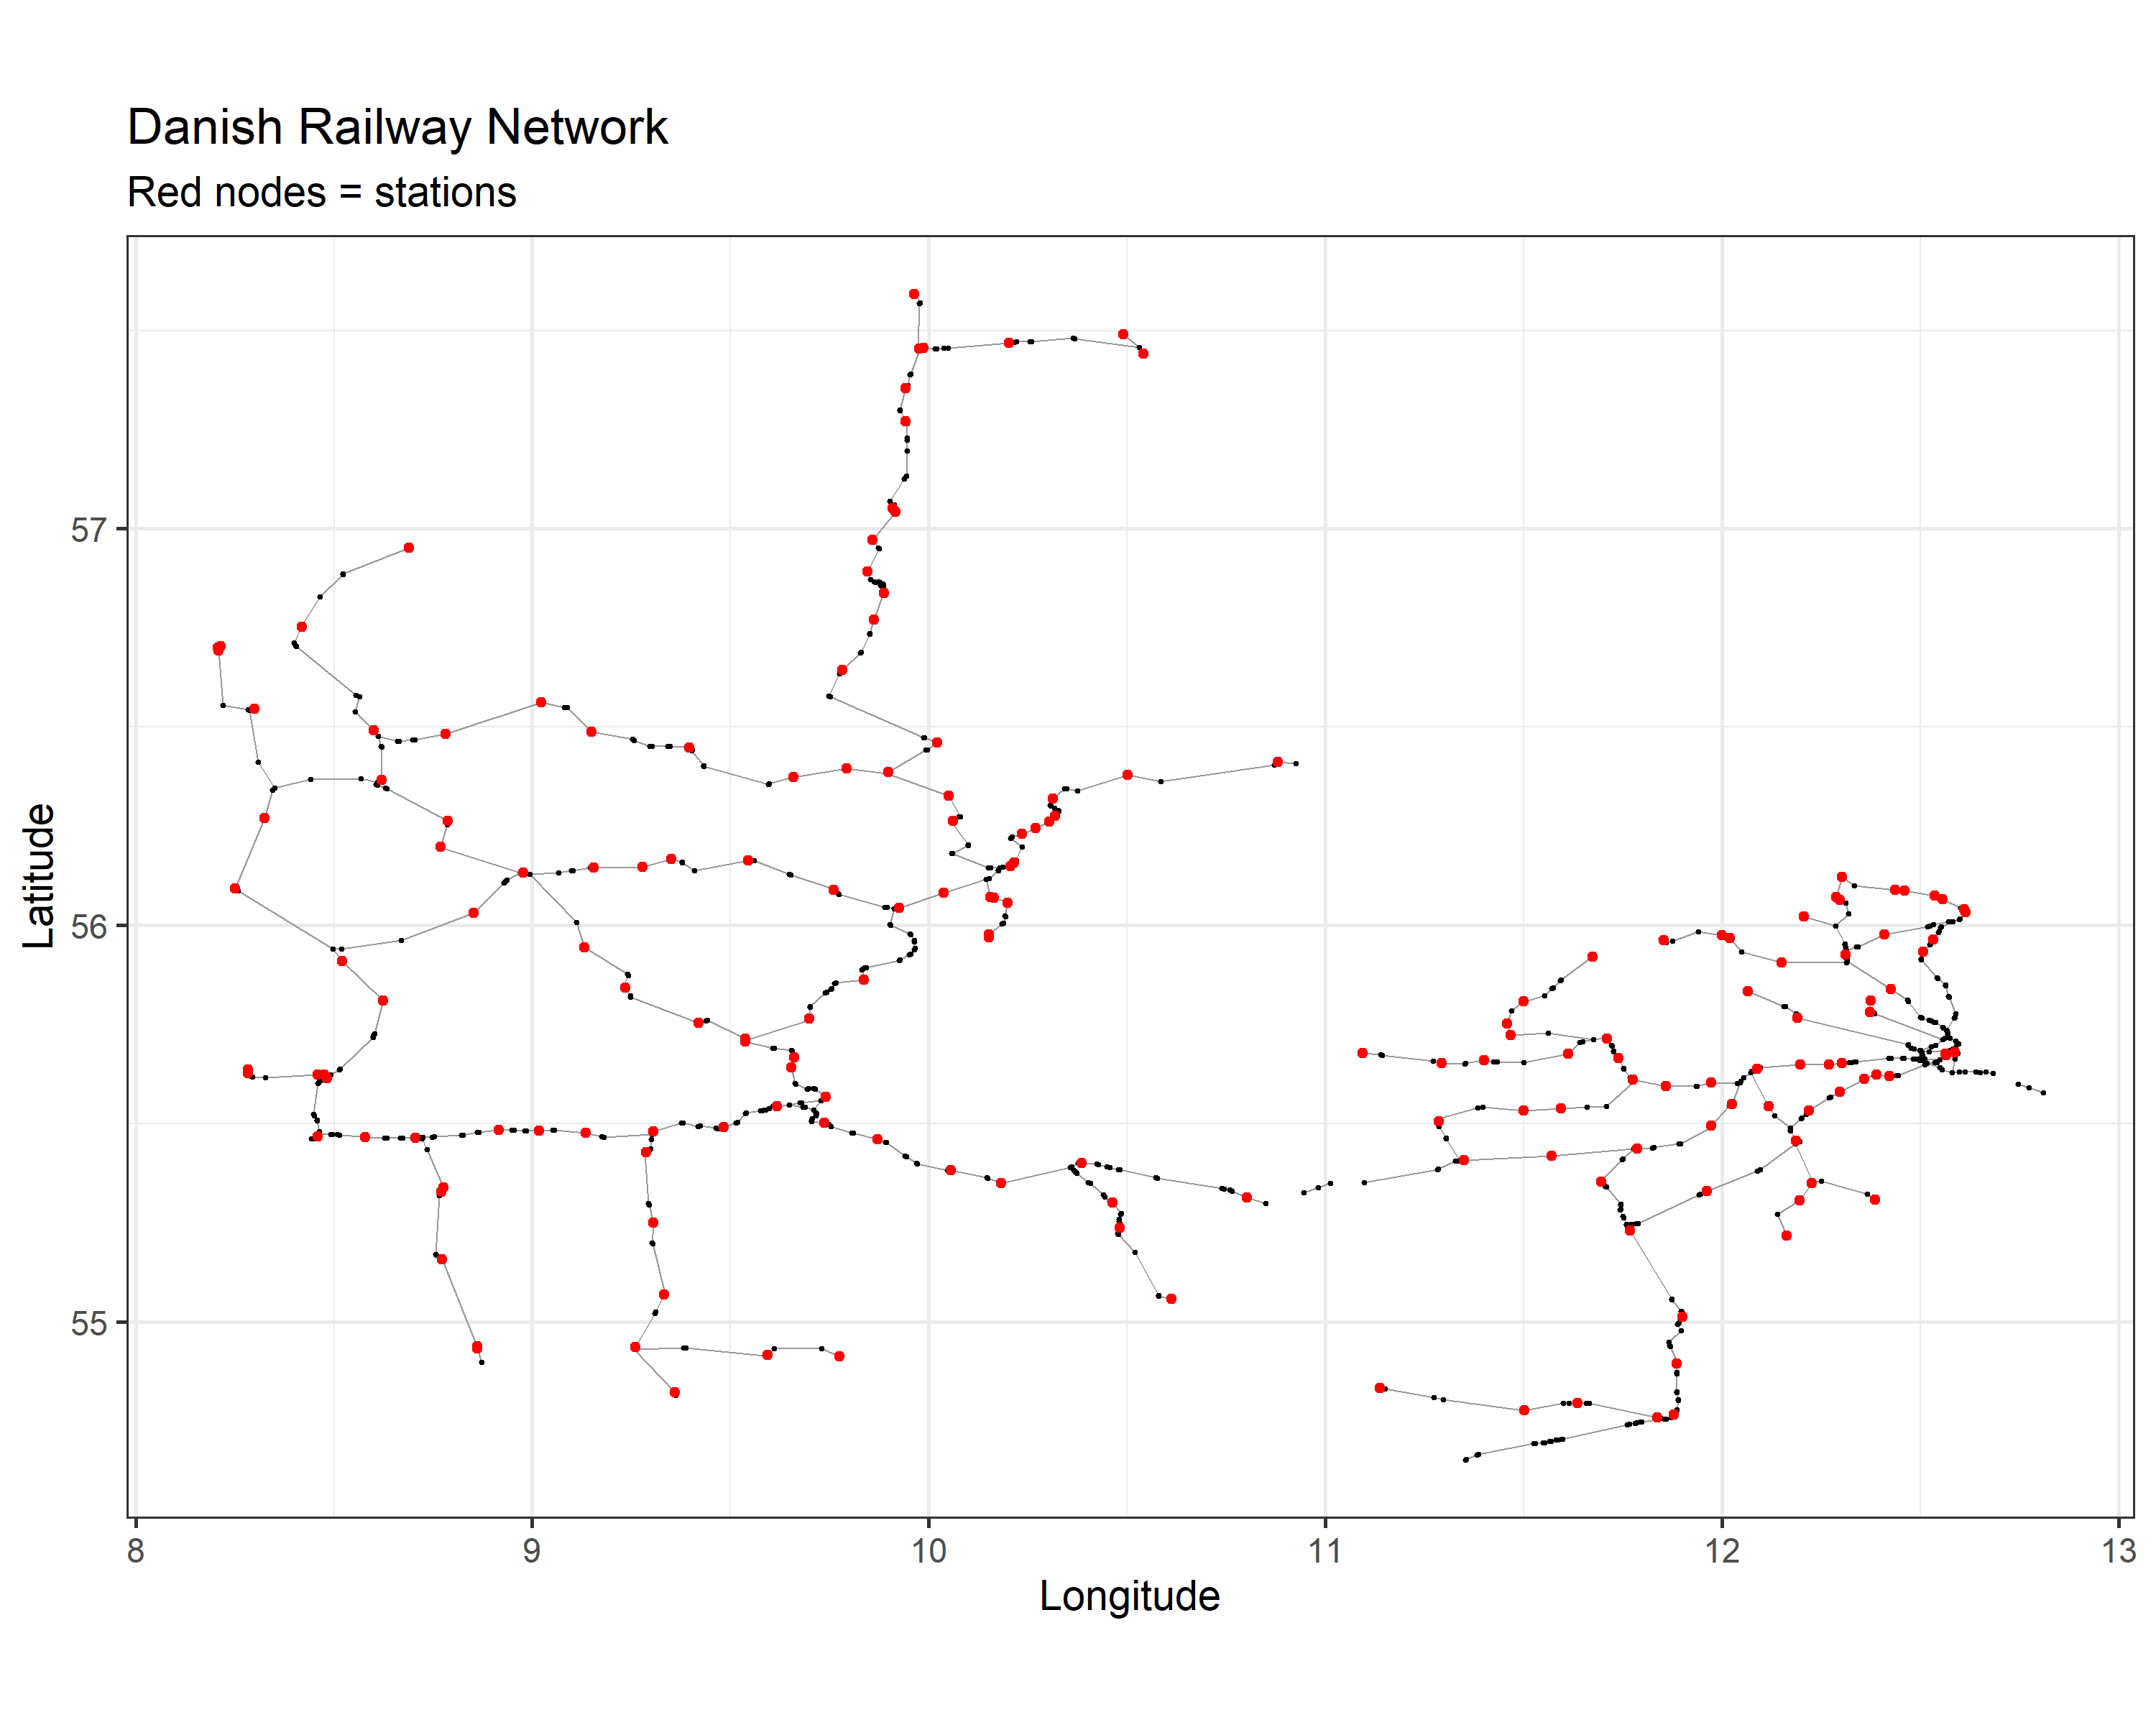
\includegraphics[width=1\textwidth]{images/railway_network_DK.png}
    }


    \caption{Danish Railways Network}
    \label{fig:dk_net}
\end{figure}





\newpage